%%% Template originaly created by Karol Kozioł (mail@karol-koziol.net) and modified for ShareLaTeX use

\documentclass[a4paper,11pt]{article}

\usepackage[T1]{fontenc}
\usepackage[utf8]{inputenc}
\usepackage{graphicx}
\usepackage{xcolor}

\renewcommand\familydefault{\sfdefault}
\usepackage{tgheros}
\usepackage[defaultmono]{droidmono}

\usepackage{amsmath,amssymb,amsthm,textcomp}
\usepackage{enumerate}
\usepackage{multicol}
\usepackage{tikz}

\usepackage{geometry}
\geometry{total={210mm,297mm},
left=25mm,right=25mm,%
bindingoffset=0mm, top=20mm,bottom=20mm}

\usepackage{subcaption}
\usepackage{float}
\usepackage{longtable}

\linespread{1.3}

\newcommand{\linia}{\rule{\linewidth}{0.5pt}}

% custom theorems if needed
\newtheoremstyle{mytheor}
    {1ex}{1ex}{\normalfont}{0pt}{\scshape}{.}{1ex}
    {{\thmname{#1 }}{\thmnumber{#2}}{\thmnote{ (#3)}}}

\theoremstyle{mytheor}
\newtheorem{defi}{Definition}

% my own titles
\makeatletter
\renewcommand{\maketitle}{
\begin{center}
\vspace{2ex}
{\huge \textsc{\@title}}
\vspace{1ex}
\\
\linia\\
\@author \hfill \@date
\vspace{4ex}
\end{center}
}
\makeatother
%%%

% custom footers and headers
\usepackage{fancyhdr}
\pagestyle{fancy}
\lhead{}
\chead{}
\rhead{}
\lfoot{Smoke Simulation}
\cfoot{}
\rfoot{Page \thepage}
\renewcommand{\headrulewidth}{0pt}
\renewcommand{\footrulewidth}{0pt}
%

% code listing settings
\usepackage{listings}
\lstset{
    language=C++,
    basicstyle=\ttfamily\small,
    aboveskip={1.0\baselineskip},
    belowskip={1.0\baselineskip},
    columns=fixed,
    extendedchars=true,
    breaklines=true,
    tabsize=4,
    prebreak=\raisebox{0ex}[0ex][0ex]{\ensuremath{\hookleftarrow}},
    frame=lines,
    showtabs=false,
    showspaces=false,
    showstringspaces=false,
    keywordstyle=\color[rgb]{0.627,0.126,0.941},
    commentstyle=\color[rgb]{0.133,0.545,0.133},
    stringstyle=\color[rgb]{01,0,0},
    numbers=left,
    numberstyle=\small,
    stepnumber=1,
    numbersep=10pt,
    captionpos=t,
    escapeinside={\%*}{*)}
}
%

%%

\setlength{\parskip}{1em}

%%

%%%----------%%%----------%%%----------%%%----------%%%

\begin{document}

\title{Smoke Simulation}

\author{Rishabh Shah, CIS 563 Physically Based Animation}

\date{05/06/2018}

\begin{figure}[H]
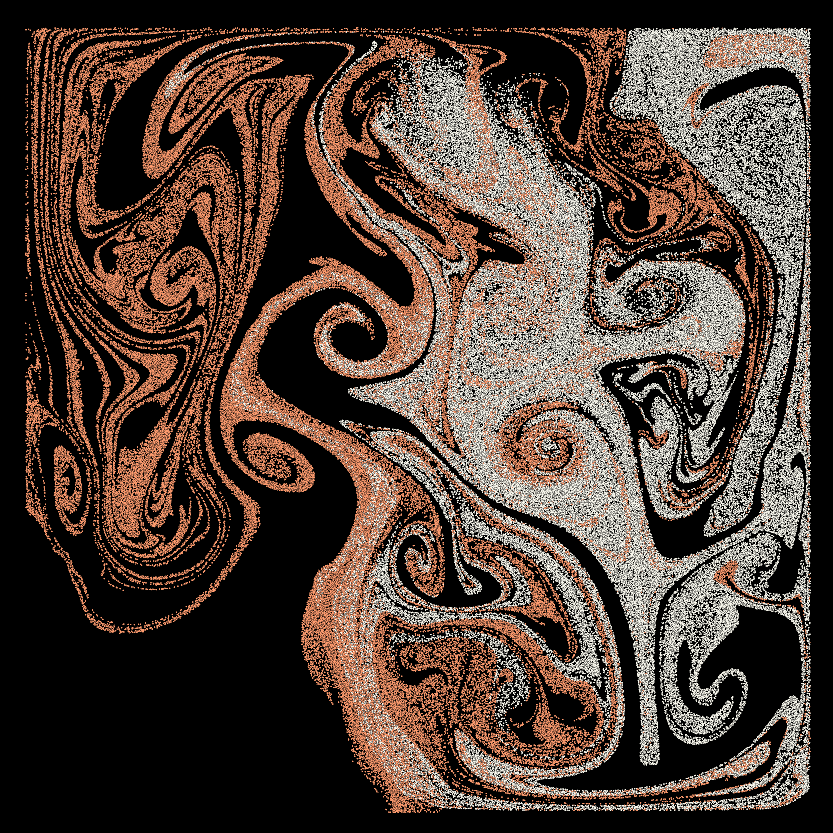
\includegraphics[width=150mm]{interacting2_5.png}
\centering
\end{figure}


\maketitle

\section*{Introduction}

With the increase in computing power, it has now become practical to simulate fluids at large scales with high physical accuracy. These simulations are used everywhere from scientific computing and research, to computer graphics applications. This project is about simulation of smoke.

\par
\noindent
The simulation uses \textbf{Semi-Lagrangian method with MAC-Grid} for simulation of smoke, with \textbf{incompressible Euler equations} and a \textbf{pressure-Poisson equation}. The model is stable for any choice of time-step. Smoke has a highly turbulent flow compared to liquid simulations, and thus it suffers from numerical dissipation, which is corrected using a \textbf{vorticity confinement term}. The implementation is able to handle boundary conditions in the simulation region, thus enabling addition of obstacles in the path of fluid flow for interesting simulations. The following sections of the readme will cover all of these components in detail.



\section*{Marker-and-Cell grid (1965, Hallow)}

For Eulerian representation in smoke simulations, MAC grid is the most used method. Here, we store different quantities at different locations. The pressure, density, temperature, etc. are stored at the cell centers, and velocities at cell faces as three separate components \textit{mU, mV, mW}. The velocity at the cell centers can be easily obtained using interpolation.



\section*{Advection}

For physical simulations, Eulerian or Lagrangian methods can be used. Eulerian method is used for smoke simulations as it is easy to handle topological changes and, collisions and interactions. But it is difficult to follow individual particles in Eulerian view, and so for advection of physical properties, we pull back and solve it like a Lagrangian problem (hence the semi-Lagrangian method). 

\par
\noindent
More specifically, for a quantity $q$, to find ${q^{n+1}(\underline{x}^*)}$, we can find an imaginary particle ${\underline{X}=\Phi^{-1}(\underline{x}^*,\Delta t)}$ at $t^n$, and grab its $Q$ value. Back tracing is used to find this imaginary particle. In this implementation, 2nd order Runga-Kutta (RK2) is used.

\par
\noindent
The example code for advection of mU (velocity in X-direction) is shown in Listing 1. Same method can be used for advecting other quantities like density and temperature also.

\begin{lstlisting}[label={list:first},caption=Sample Advection code -- Advecting velocities in X-direction i.e. mU]
FOR_EACH_FACE {
    // Check if the face is valid
    if (isValidFace(MACGrid::X, i, j, k)) { 
        // get current face position
        vec3 currentPt = getFacePosition(MACGrid::X, i, j, k); 
        
        // back trace and get the old position of the imaginary particle 
        vec3 oldPt = getRewoundPosition(currentPt, dt);
        
        // get the velocity at old position
        vec3 newVel = getVelocity(oldPt);
        
        // update the current mU
        target.mU(i, j, k) = newVel[0]; 
    }
    mU = target.mU; // using target as a temporary buffer
}
\end{lstlisting}




\section*{External Forces}

To make the simulation look realistic, we need to add external environmental forces like gravity and buoyancy. It is done as shown in listing 2. Here, \textit{theBuoyancyAlpha} controls the effect of gravity on the smoke. It is multiplied with density as it represents the mass in unit volume of the grid cell, and is obviously in the downward direction (hence the negative sign). \textit{theBuoyancyBeta} controls the effect of buoyancy due to the temperature difference with the surrounding environment.

\begin{lstlisting}[label={list:second},caption= Buoyancy and Gravity]
FOR_EACH_FACE{
    // Check if the face is valid
    if(isValidFace(MACGrid::Y, i, j, k)) {
        // get current face position
        vec3 facePos = getFacePosition(MACGrid::Y, i, j, k);
        
        // compute the overall effect of buoyancy and gravity
        double temperatureDifference = 
            getTemperature(facePos) - theBuoyancyAmbientTemperature;
            
        double buoyancy = - theBuoyancyAlpha * getDensity(facePos) 
                          + theBuoyancyBeta * temperatureDifference;
                          
        // update the Y-velocity as per the buoyancy
        target.mV(i, j, k) += dt * buoyancy;
    }
}
\end{lstlisting}

\par
\noindent
As stated in the introduction, the fluid solver is dissipative and so we need a way to get that energy back in the system. The dissipation here is of rotational energy, and we add that back using \textit{vorticity confinement term} as an external force. 

\par
\noindent
The steps for computing vorticity confinement can be summarized as follows:
\begin{enumerate}
    \item Compute velocity at cell centers. 
        This can be done simply by averaging velocities at surrounding faces.
        \tiny
        \begin{verbatim}
        FOR_EACH_CELL {
            u(i, j, k) = (mU(i + 1, j, k) + mU(i, j, k)) / 2;
            v(i, j, k) = (mV(i, j + 1, k) + mV(i, j, k)) / 2;
            w(i, j, k) = (mW(i, j, k + 1) + mW(i, j, k)) / 2;
        }
        \end{verbatim}
        \normalsize
    \item Compute vorticities at cell centers using central derivatives.
        \tiny
        \begin{verbatim}  
        double inv2h = 1.0 / (2.0 * theCellSize);
        FOR_EACH_CELL {
            vorticityX(i, j, k) = inv2h * (w(i, j + 1, k) - w(i, j - 1, k) - v(i, j, k + 1) + v(i, j, k - 1));
            vorticityY(i, j, k) = inv2h * (u(i, j, k + 1) - u(i, j, k - 1) - w(i + 1, j, k) + w(i - 1, j, k));
            vorticityZ(i, j, k) = inv2h * (v(i + 1, j, k) - v(i - 1, j, k) - u(i, j + 1, k) + u(i, j - 1, k));
            vorticityLen(i, j, k) = vec3(vorticityX(i, j, k), vorticityY(i, j, k), vorticityZ(i, j, k)).Length();
        }
        \end{verbatim}  
        \normalsize
    \item Compute vorticity gradient and normalize it to get N. Cross product of N and vorticity is used to compute the final force. This is used to update the velocities at cell faces.
        \tiny
        \begin{verbatim}
        FOR_EACH_CELL {
            vec3 vortGrad(vorticityLen(i+1, j, k) - vorticityLen(i-1, j, k),
                          vorticityLen(i, j+1, k) - vorticityLen(i, j-1, k),
                          vorticityLen(i, j, k+1) - vorticityLen(i, j, k-1));
            vortGrad *= inv2h;
    
            vec3 N = vortGrad.Normalize();
    
            vec3 fconf = theVorticityEpsilon * theCellSize *
                         N.Cross(vec3(vorticityX(i, j, k), vorticityY(i, j, k), vorticityZ(i, j, k)));
    
            // Apply vortcity confinement to faces..
            // X
            if(isValidFace(MACGrid::X, i, j, k)) {
                target.mU(i, j, k) += dt * fconf[0]/2;
            }
            //// SIMILAR FOR Y AND Z ////
            
            // X+1
            if(isValidFace(MACGrid::X, i+1, j, k)) {
                target.mU(i+1, j, k) += dt * fconf[0]/2;
            }
            //// SIMILAR FOR Y+1 AND Z+1 ////
        }
        \end{verbatim}
        \normalsize
\end{enumerate}




\section*{Projection}

The projection step in our algorithm is where pressure is computed and updated, and the resultant effect on velocities is reflected in the MAC grid. The steps for computing pressure projection are as follows:

\begin{enumerate}
    \item Compute the divergence at cell centers. A boundary condition is used here to make sure the cells outside the simulation domain are not used for calculations.
        \tiny
        \begin{verbatim}
        FOR_EACH_CELL {
            double velLowX = (i > 0) ? mU(i, j, k) : 0.0;
            double velHighX = (i + 1 < theDim[MACGrid::X]) ? mU(i + 1, j, k) : 0.0;
            double velLowY = (j > 0) ? mV(i, j, k) : 0.0;
            double velHighY = (j + 1 < theDim[MACGrid::Y]) ? mV(i, j + 1, k) : 0.0;
            double velLowZ = (k > 0) ? mW(i, j, k) : 0.0;
            double velHighZ = (k + 1 < theDim[MACGrid::Z]) ? mW(i, j, k + 1) : 0.0;
            d(i, j, k) = -((velHighX - velLowX) + (velHighY - velLowY) + (velHighZ - velLowZ)) / theCellSize;
        }
        \end{verbatim}
        \normalsize
    \item Compute pressure at cell centers using Preconditioned Conjugate Gradient algorithm
        \tiny
        \begin{verbatim}
        preconditionedConjugateGradient(AMatrix, p, d, 200, 0.01);
        FOR_EACH_CELL {
            p(i, j, k) *= constMultiplier;
        }
        \end{verbatim}
        \normalsize
    \item Update velocities using updated pressure.
        \tiny
        \begin{verbatim}
        double constMultiplier1 = dt / (theAirDensity * theCellSize);
        FOR_EACH_FACE {
            // X
            if (isValidFace(MACGrid::X, i, j, k)) {
                if (isValidCell(i - 1, j, k) && isValidCell(i, j, k)) {
                    double deltaPX = p(i, j, k) - p(i - 1, j, k);
                    target.mU(i, j, k) -= constMultiplier1 * deltaPX;
                }
                else{
                    target.mU(i, j, k) = 0.0;
                }
            }
            //// SIMILAR FOR Y AND Z ////
        }
        \end{verbatim}
        \normalsize
        
\end{enumerate}


\section*{Simulation Algorithm}

Using all the above concepts, we can summarize each step of the algorithm as follows:
\begin{lstlisting}
void SmokeSim::step() {
    // time step size
    double dt = 0.1;
    
    // update the sources - inject smoke into the system
    mGrid.updateSources();
    
    // advect velocity
    mGrid.advectVelocity(dt);
    
    // add gravity, buoyancy, and vorticity confinement
    mGrid.addExternalForces(dt);
    
    // projection step
    mGrid.project(dt);
    
    // advect temperature
    mGrid.advectTemperature(dt);
    
    // advect density
    mGrid.advectDensity(dt);
    
    // advect rendering particles for visualization
    mGrid.advectRenderingParticles(dt);
    
    mTotalFrameNum++;
}
\end{lstlisting}


\section*{Multi-threading}

As the grid based simulation has a lot of components that can be parallelized, I have added multi-threading to the main simulation code functions such that the simulation can run on 4 threads. Note that only the functions of the simulation step (see previous section) are parallel, the main thread still has to do a lot of extra work in between steps, and for the opengl rendering. So the performance boost is not easily evident. But the simulation step is about 25\% faster. This is useful when the opengl preview is not used and only the simulation frames are written out to files. Multithreading only works when grid resolution in Z direction is atleast 4.


\section*{Results}

The comparison between smoke with different density and temperature values can be seen in Table 2. 

\begin{table}[H]
\caption{Legend for images in Table 2}
\centering
\begin{tabular}{cc}
d=0.3, t=1.0 & d=0.9, t=1.0\\
\newline
d=0.3, t=3.0 & d=0.9, t=3.0\\
\end{tabular}
\end{table}

\begin{table}[H]
\caption{Density and temperature comparison}
\centering
\begin{tabular}{cc}
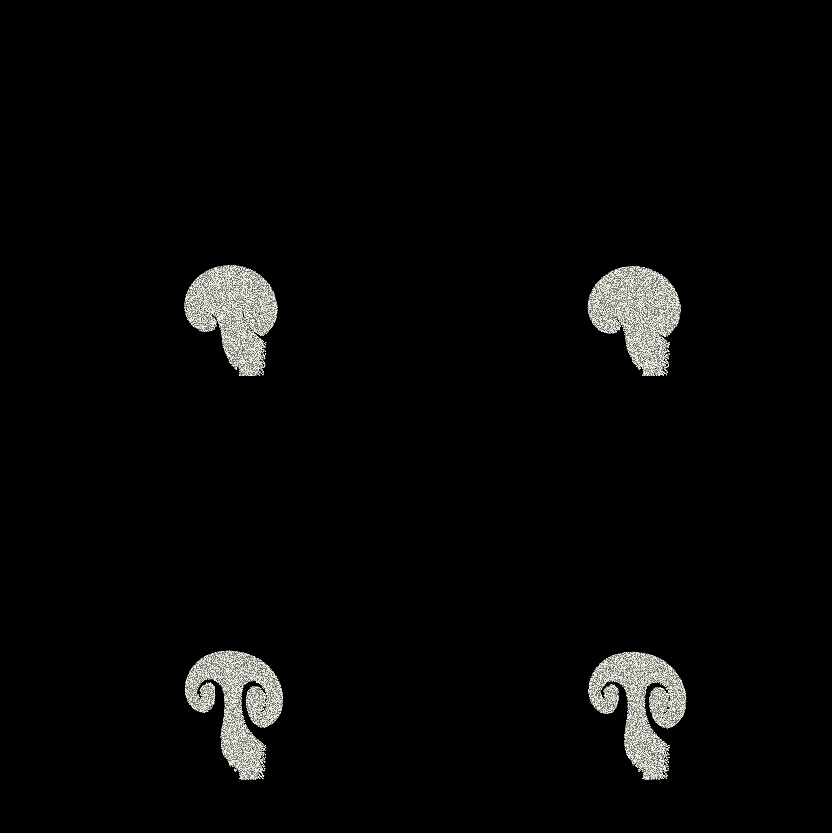
\includegraphics[width=70mm]{comp_60.png} &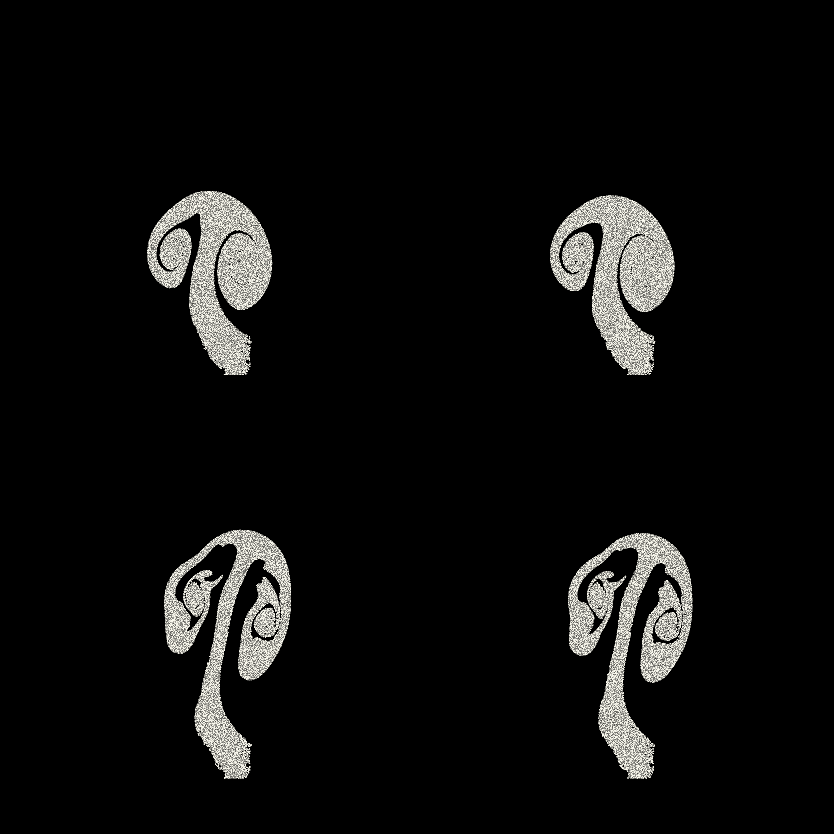
\includegraphics[width=70mm]{comp_120.png}\\
\newline
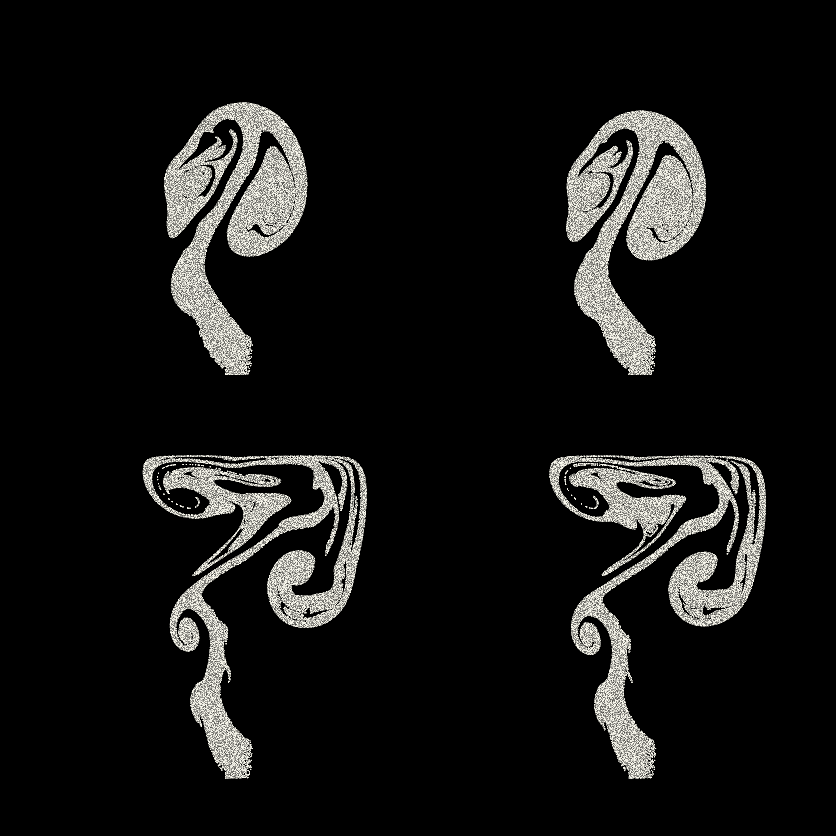
\includegraphics[width=70mm]{comp_180.png}&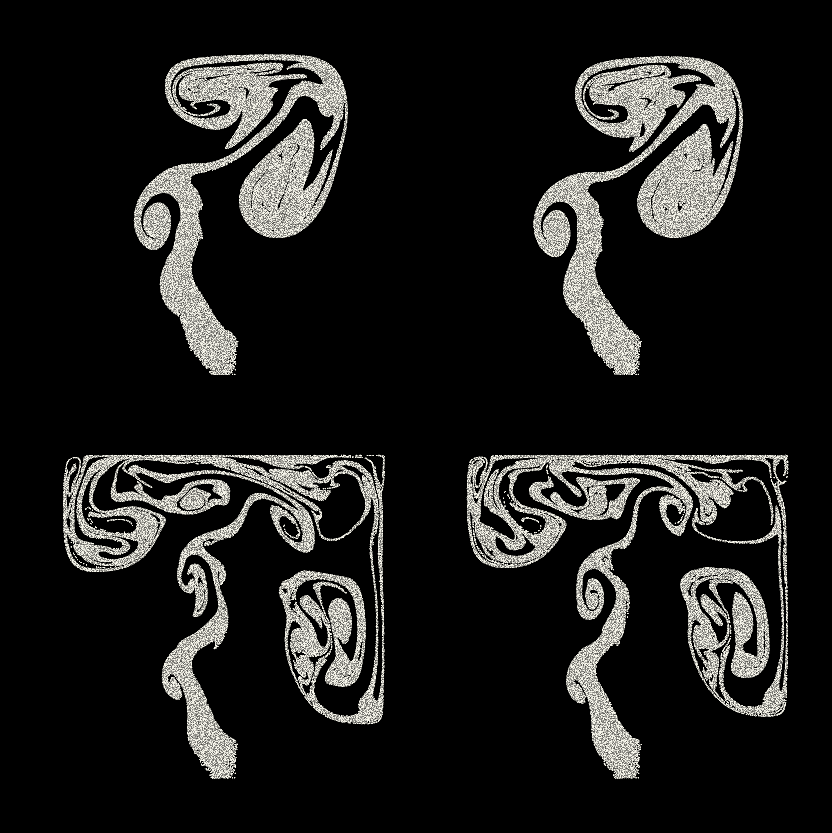
\includegraphics[width=70mm]{comp_240.png}\\
\newline
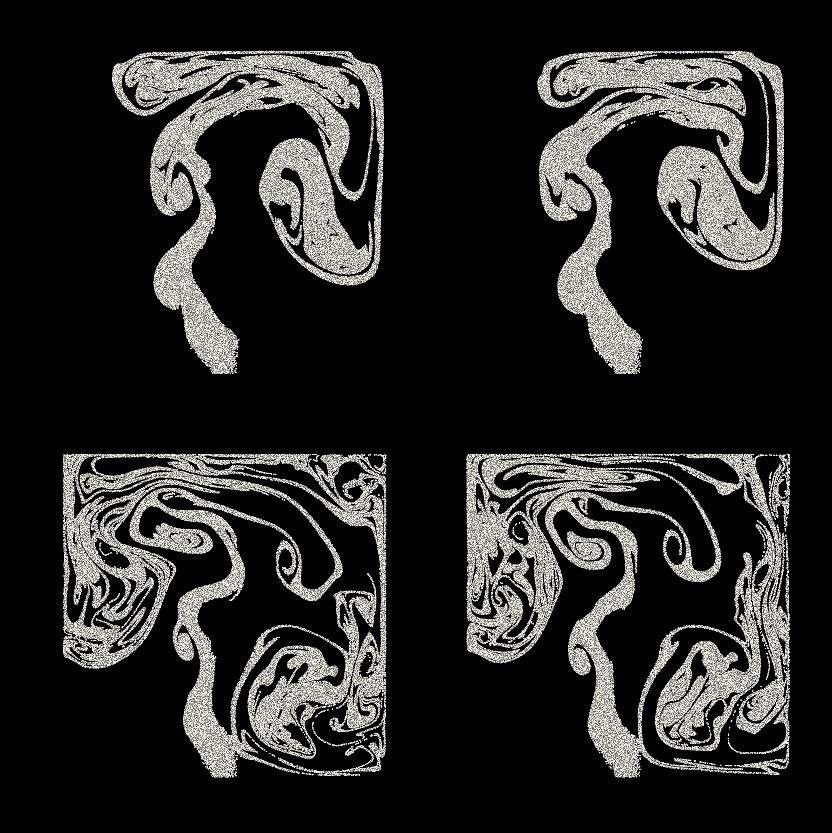
\includegraphics[width=70mm]{comp_300.png}&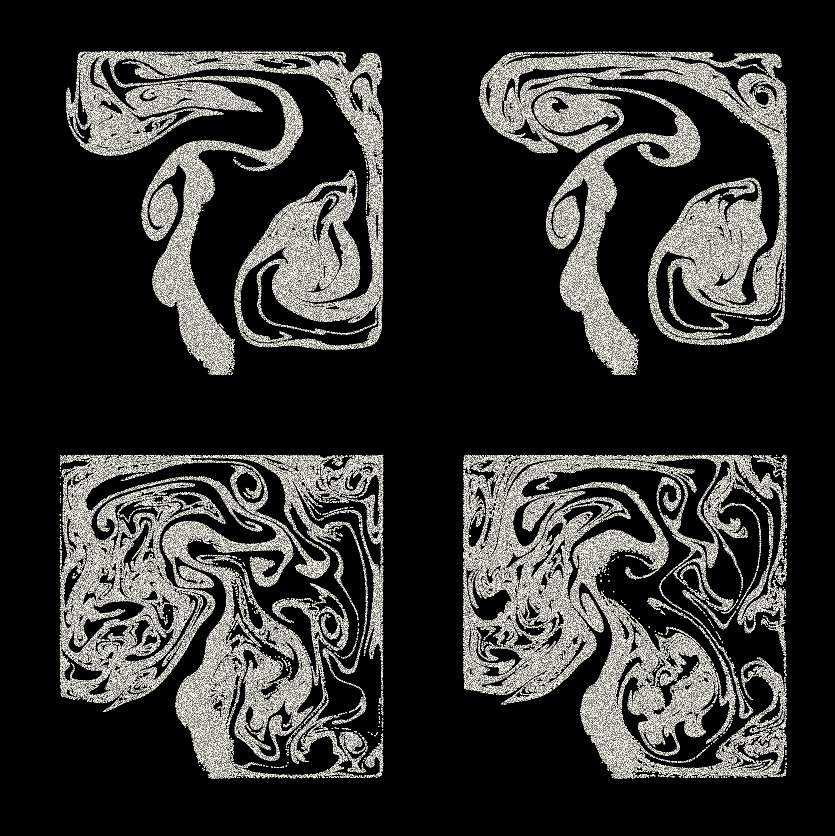
\includegraphics[width=70mm]{comp_360.png}\\
\end{tabular}
\end{table}


\par
\noindent
I added ability to give colors to smoke particles for visualization on smoke interaction in Houdini. In Table 3, two smokes of different temperatures can be seen merging.

\begin{table}[H]
\caption{Merging smoke with different temperatures}
\centering
\begin{tabular}{cc}
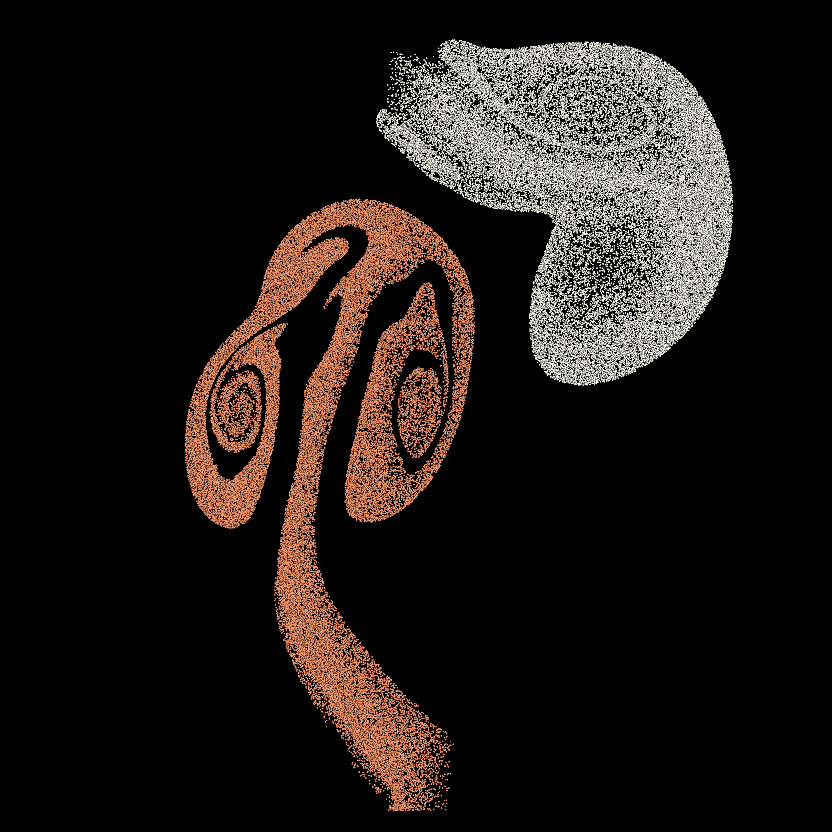
\includegraphics[width=70mm]{interacting2_2.png} &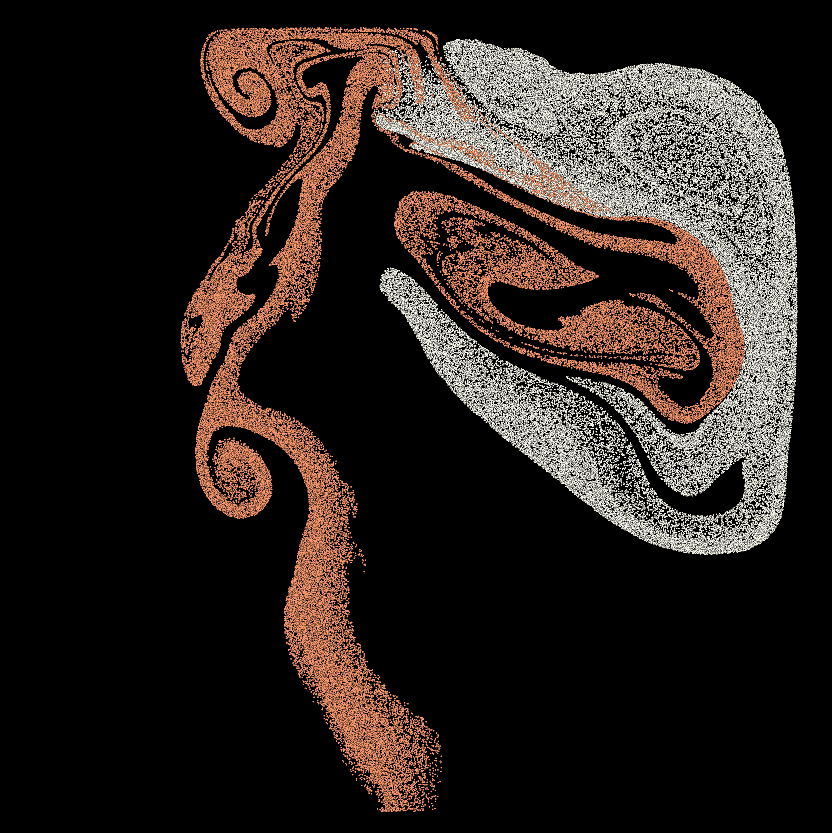
\includegraphics[width=70mm]{interacting2_3.png}\\
\newline
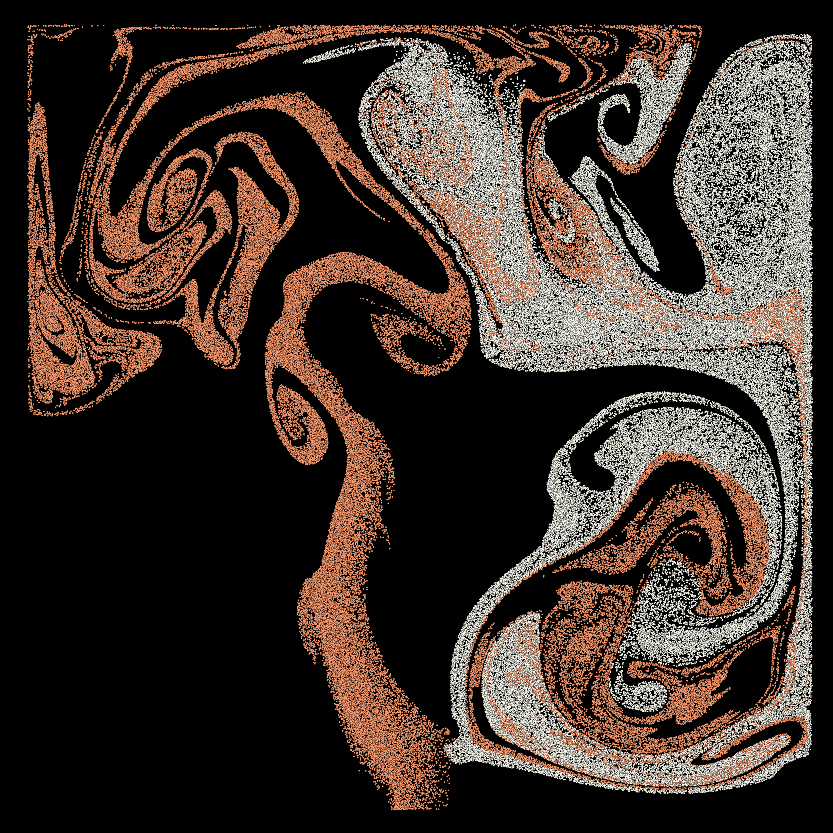
\includegraphics[width=70mm]{interacting2_4.png}&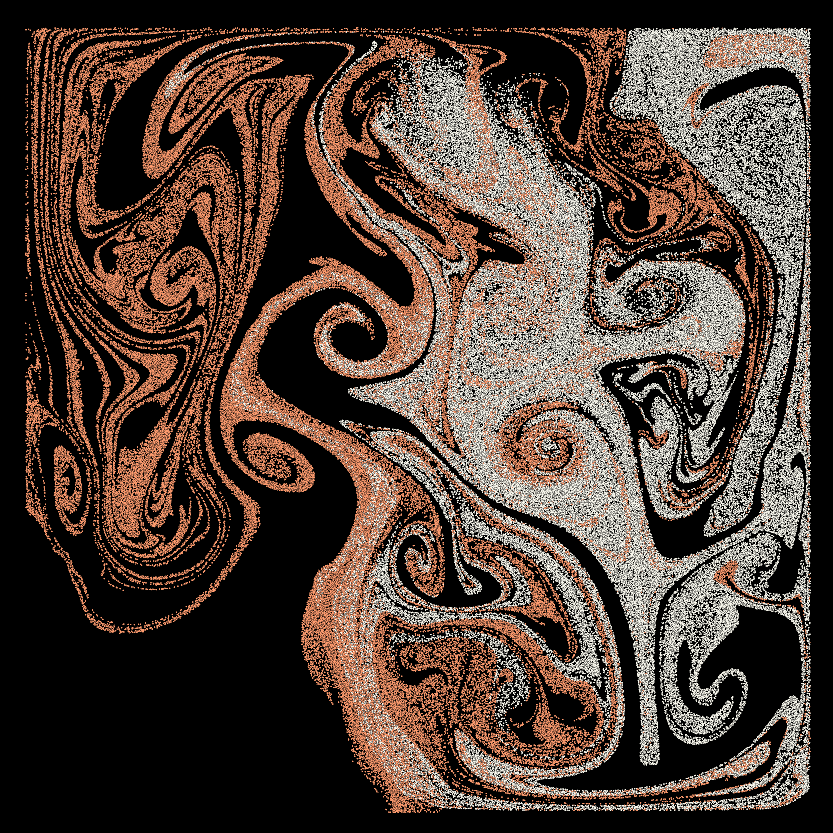
\includegraphics[width=70mm]{interacting2_5.png}\\
\end{tabular}
\end{table}


\par
\noindent
Another example of merging smokes is in Table 4. Here, the sources produce exactly same smoke but with velocities in different directions and with different colors. This simulation is in 3D.

\begin{table}[H]
\caption{Merging smoke}
\centering
\begin{tabular}{cc}
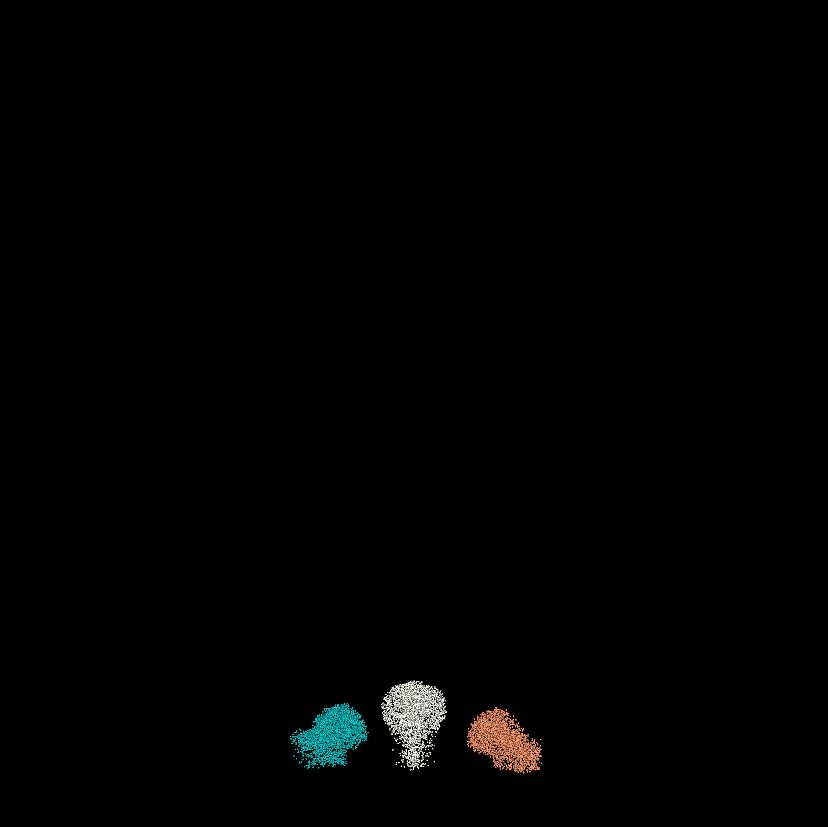
\includegraphics[width=70mm]{interacting_1.png} &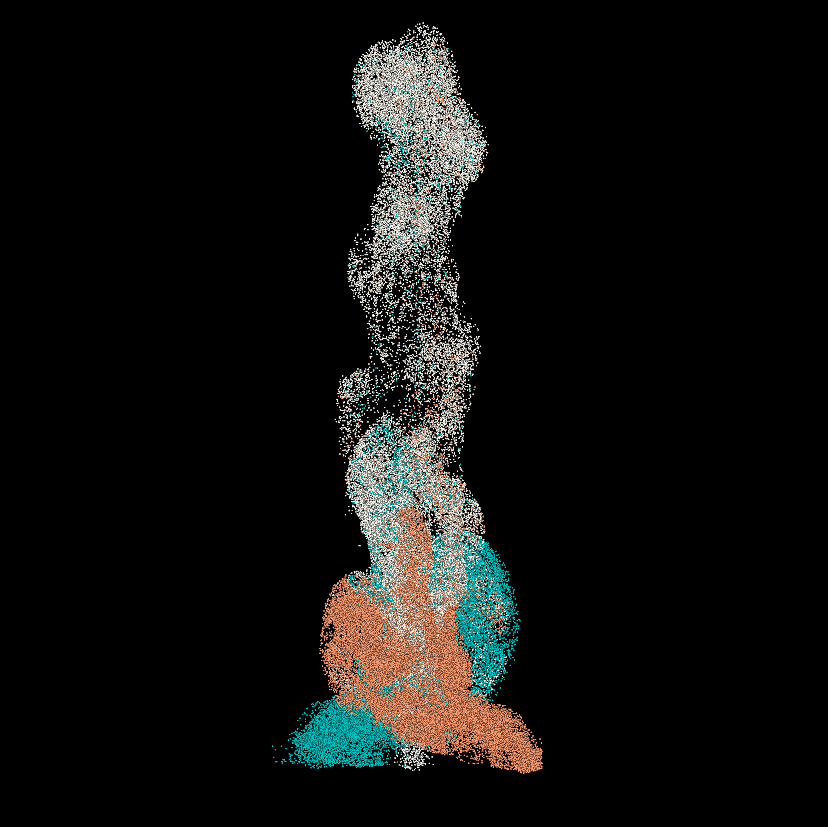
\includegraphics[width=70mm]{interacting_2.png}\\
\end{tabular}
\end{table}



\par
\noindent
The example in Table 5 shows various frames of smoke interacting with obstacles (like a grid of cubes) placed above the source. The images are from the top view of the 3D simulation. Both density and particle views are shown side by side.

\begin{table}[H]
\caption{Interaction with obstacles - Top view}
\centering
\begin{tabular}{cc}
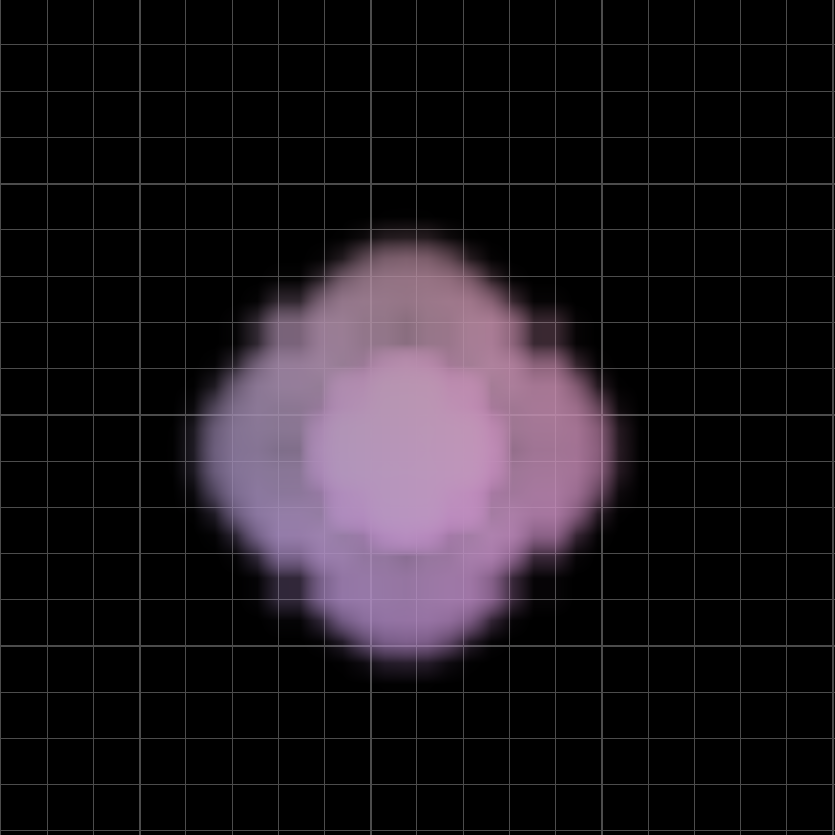
\includegraphics[width=70mm]{obs_d_2.png} &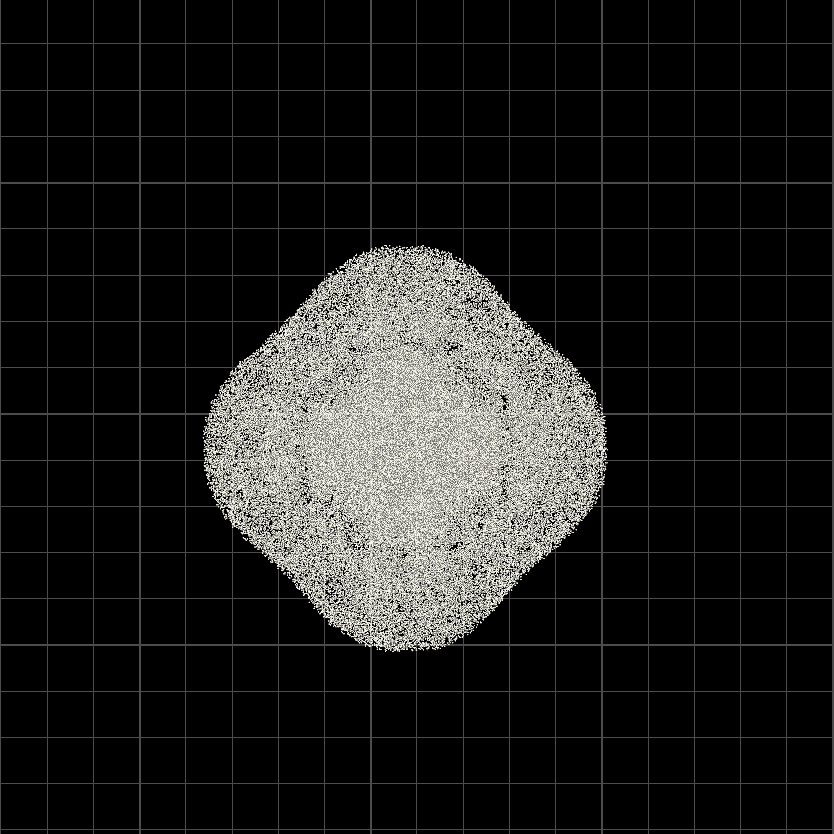
\includegraphics[width=70mm]{obs_p_2.png}\\
\newline
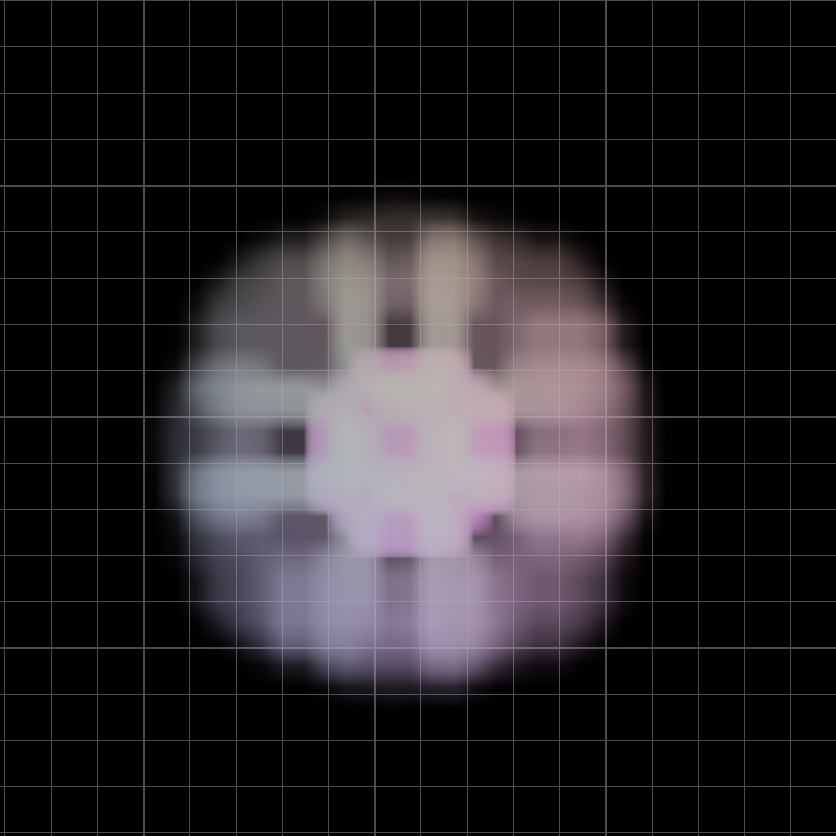
\includegraphics[width=70mm]{obs_d_3.png} &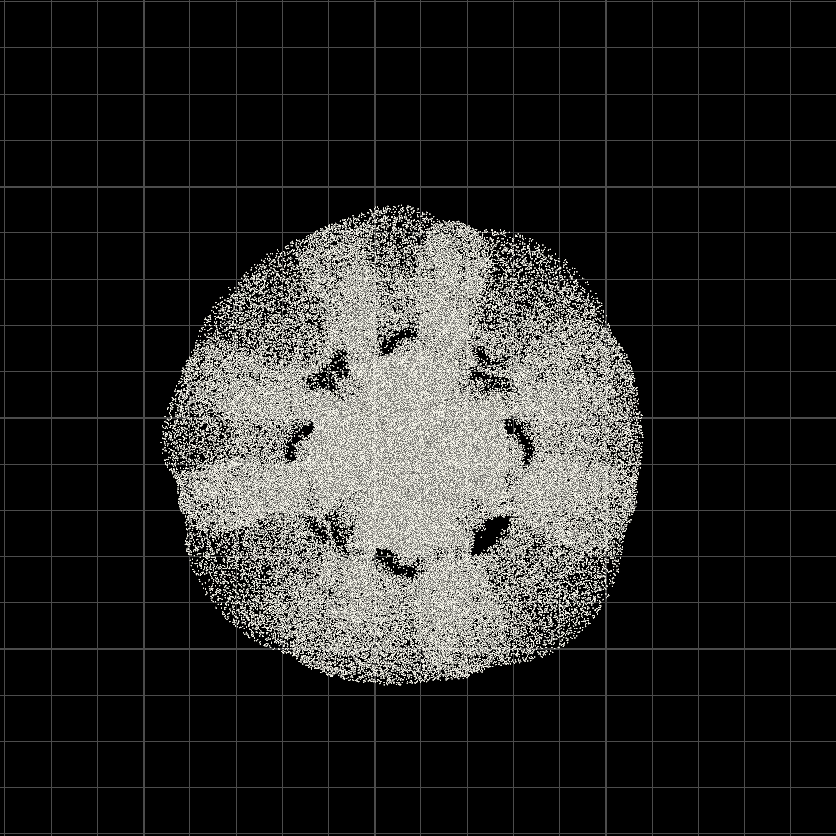
\includegraphics[width=70mm]{obs_p_3.png}\\
\newline
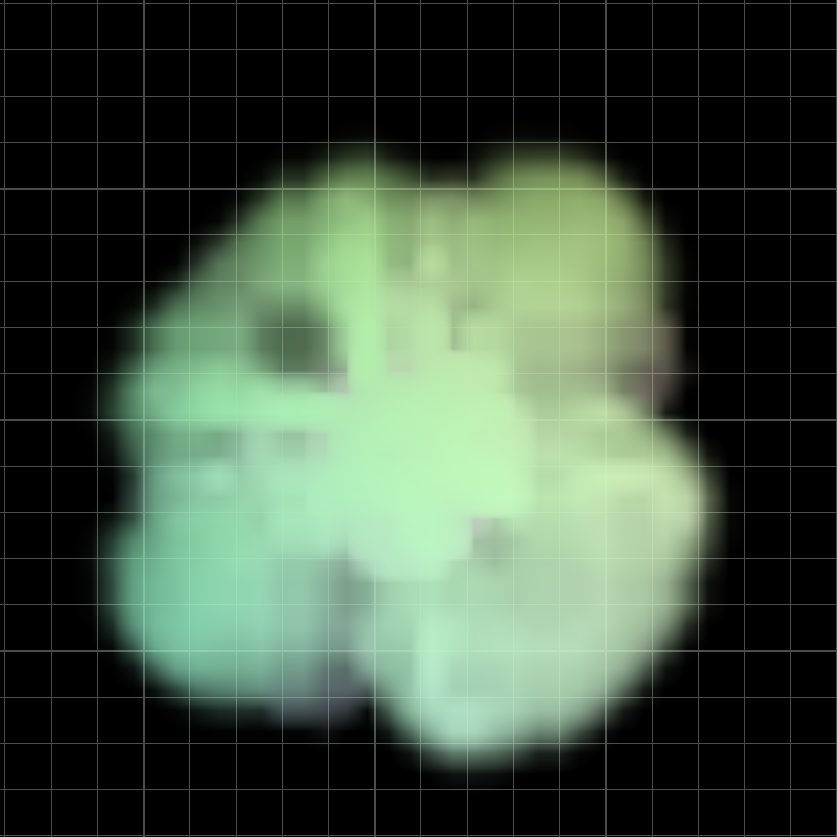
\includegraphics[width=70mm]{obs_d_5.png} &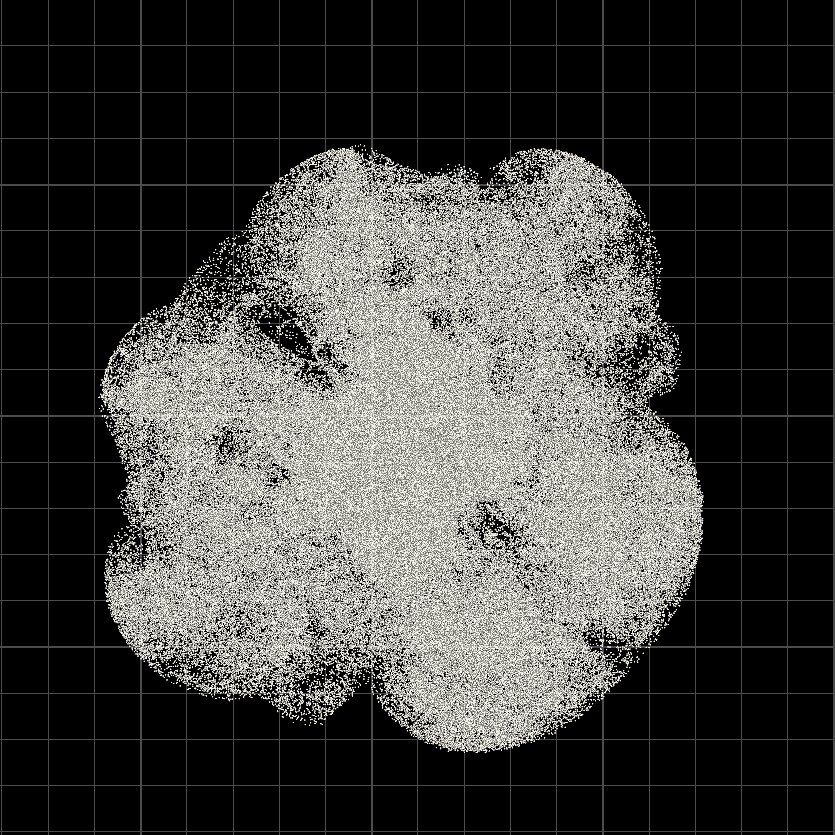
\includegraphics[width=70mm]{obs_p_5.png}\\
\end{tabular}
\end{table}


\par
\noindent
Videos of these simulations and some other interesting demos can be found along with the submission. 


\section*{References}
\begin{enumerate}
    \item "Visual Simulation of Smoke", Ronald Fedkiw, Jos Stam, Henrik Wann Jensen
    \item "Fluid Simulation SIGGRAPH 2007 Course Notes", Robert Bridson, Matthias Müller-Fischer
\end{enumerate}


%%%%%%%%%%%%%%%%%%%%%%%%%%%%%%%%%%%%%%%%%%%%%555
\end{document}
